\section{Durchführung}

% wichtige zitierte wie \cite{nunes_systematic_2017} wurden trotzdem genommen.

Nach der initialen Suche wurden mehrere Filterschritte durchgeführt. \autoref{fig:04_literature_review_selection_process} bietet einen Überblick über das Auswahlverfahren der Arbeiten, auf denen die hier entstandenen Ergebnisse aufbauen. Der Auswahlprozess ist in drei Iterationen erfolgt. Die Suche in den vier vorgestellten Datenbanken hat insgesamt 790 Ergebnisse ergeben. Dabei gab es 141 Duplikate. Die initiale Menge nach der Suche enthielt folglich 649 wissenschaftliche Arbeiten. Da die Suche auf die genannten vier Datenbanken beschränkt passenden Filter genutzt wurden, erfüllen diese Veröffentlichungen bereits die Kriterien des \textit{Peer Reviews}([IC1]).

\begin{figure}[htb]
    \centering
    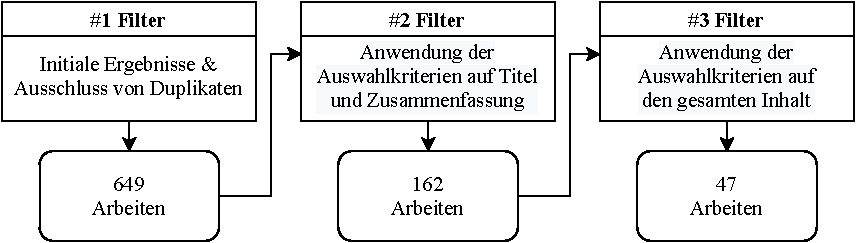
\includegraphics[width=\textwidth]{contents/04_literature_review/res/selection_process.pdf}
    \caption{Auswahlverfahren der Literaturrecherche}
    \label{fig:04_literature_review_selection_process}
\end{figure}

In einem zweiten Schritt wurden die Selektionskriterien auf den Titel und die Zusammenfassung der Arbeiten angewendet. Für die übrigen 162 Veröffentlichungen wurde der Volltext auf die Kriterien überprüft, wobei am Ende 47 Arbeiten alle Selektionskriterien erfüllt haben. Im Anschluss an die Auswahl wurden neun weitere Ergebnisse aufgenommen, die zum Verständnis einer anderen Arbeit wichtig waren und ebenfalls die Selektionskriterien erfüllt haben. Final enthält die Menge der wissenschaftlichen Arbeiten, die als Informationsgrundlage für die Erstellung eines Leitfadens zur Integration von Erklärungen gedient hat 56 Arbeiten.